\chapter{Inference Adaptation}
\chaptermark{Inference Adaptation}
\label{chap:inference_adaptation}

Extending the tokenizer with new tokens enables more efficient representation of Portuguese text but also introduces challenges, since the model has never encountered these tokens during pre-training, which may result in incoherent or repetitive outputs.

This chapter introduces an inference adaptation framework designed to mitigate this problem.

\section{Motivation}

To understand the need for a specialized inference procedure, we performed stepwise experiments illustrating the evolution of model behavior.

All experiments in this chapter were conducted using the following model configuration:
\begin{itemize}
    \item \textbf{Model:} HuggingFaceTB/SmolLM2-135M
    \item \textbf{Tokenizer (BPE) Dataset:} OpenSubtitles\footnote{OpenSubtitles Corpus: \url{https://opus.nlpl.eu/results/en&pt/corpus-result-table}}, sample of 1000 datapoints
    \item \textbf{Number of Added Tokens:} 10,000
    \item \textbf{Embeddings Initialization Method:} \texttt{weighted\_drop(1.5)}
    \item \textbf{Maximum New Tokens:} 20
\end{itemize}


\subsection{Baseline Generation}
We first tested the model using its original tokenizer and weights (Table~\ref{tab:default-baseline}) without adding any new tokens. This baseline demonstrates how the pre-trained model performs on Portuguese prompts prior to any modifications.

\begin{table}[H]
    \centering
    \begin{tabular}{|p{0.3\linewidth}|p{0.6\linewidth}|}
        \hline
        \textbf{Prompt} & \textbf{Generated Output (Original Tokenizer)} \\
        \hline
        Olá, podes contar-me um poema com as palavras: Sol, Lua, Céu e Nuvens? & Ao fazer isso, o poeta deve ter uma palavra \\
        \hline
        Bacalhau é um dos peixes mais utilizados na culinária & Ao entender a criatura dos peixes, o uso de \\
        \hline
    \end{tabular}
    \caption{Baseline generation}
    \label{tab:default-baseline}
\end{table}

\subsection{Default Inference Generation After Tokenizer Adaptation}
Next, we added 10,000 Portuguese-specific tokens to the tokenizer. Using the default inference procedure with the expanded tokenizer, the model produced incoherent generations, as shown in Table~\ref{tab:default-inference-results}. This highlights the limitations of simply adding tokens without modifying inference.

\begin{table}[H]
    \centering
    \begin{tabular}{|p{0.3\linewidth}|p{0.6\linewidth}|}
        \hline
        \textbf{Prompt} & \textbf{Generated Output (Default Inference)} \\
        \hline
        Olá, podes contar-me um poema com as palavras: Sol, Lua, Céu e Nuvens? & Ao que o que o que o que o que o que o que o que o \\
        \hline
        Bacalhau é um dos peixes mais utilizados na culinária & de alimentos. Ao entender a dieta dos alimentos, o \\
        \hline
    \end{tabular}
    \caption{Adapted model default inference generation}
    \label{tab:default-inference-results}
\end{table}

\section{Proposed Inference Framework}
To address the problems observed in the previous step, we developed a two-phase inference adaptation procedure:

\begin{enumerate}
    \item \textbf{Input Processing}: Input text is first tokenized using the original tokenizer, allowing the model to leverage its pre-trained distribution.
    \item \textbf{Output Processing}: If the model generates a newly added token, it is dynamically replaced with its constituent original tokens before being fed back into the model.
\end{enumerate}

This ensures compatibility with the pre-trained distribution while preserving token efficiency gains. An algorithmic proposal for this approach follows:

\textbf{Proposed Algorithm}
\begin{lstlisting}
def inference(model, tokenizer, encoding_tokenizer, prompt):
    outputs = []
    for i in range(max_new_tokens):
        if len(outputs) > 0:
            inputs = encoding_tokenizer.encode(prompt + tokenizer.decode(outputs))
        new_token = model.generate(input_ids, max_new_tokens=1)
        outputs.append(new_token)
    generation = tokenizer.decode(outputs)
    return generation
\end{lstlisting}

\begin{figure}[h]
    \centering
    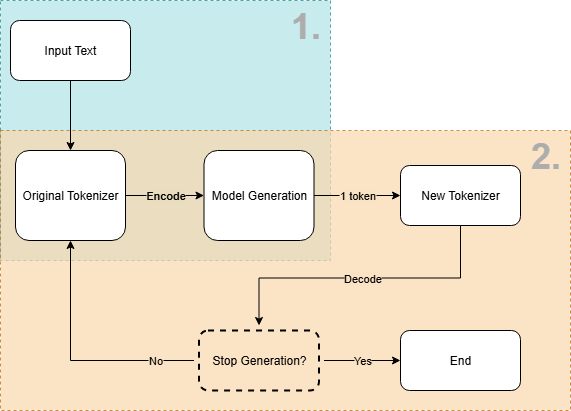
\includegraphics[width=0.8\linewidth]{Figures/Inference Adaptation.png}
    \caption{Inference Adaptation Framework}
    \label{fig:inference-adaptation}
\end{figure}

\section{Implementation Considerations}
The current implementation was developed at the Python level using the Hugging Face Transformers library. For production-level deployment, future work would require:

\begin{itemize}
    \item Optimization of the inference process to minimize computational overhead.
    \item Development of custom extensions within \texttt{PyTorch} to natively handle dynamic token mapping.
\end{itemize}

\section{Potential Benefits}
If implemented at a lower level, inference adaptation could yield several benefits:

\begin{itemize}
    \item \textbf{Improved Generation Coherence}: Reduce inconsistencies when generating text with new tokens. (See \S\ref{sec:results_new_inference})
 
    \item \textbf{Enhanced Token Efficiency}: The approach would preserve the token efficiency
gains of extending the vocabulary, while mitigating impacts on model effectiveness.

\end{itemize}

\section{Illustrative Results}
\label{sec:results_new_inference}
After applying the inference framework, coherence for the same prompts is now restored, as shown in Table~\ref{tab:adapted-inference-results}:

\begin{table}[H]
    \centering
    \begin{tabular}{|p{0.3\linewidth}|p{0.6\linewidth}|}
        \hline
        \textbf{Prompt} & \textbf{Generated Output (With Inference Adaptation)} \\
        \hline
        Olá, podes contar-me um poema com as palavras: Sol, Lua, Céu e Nuvens? & Ao fazer isso, o poeta deve ter uma palavra \\
        \hline
        Bacalhau é um dos peixes mais utilizados na culinária & Ao entender a criatura dos peixes, o uso de \\
        \hline
    \end{tabular}
    \caption{Preliminary test outputs using the proposed inference adaptation with expanded tokenizer}
    \label{tab:adapted-inference-results}
\end{table}

These results confirm that the framework preserves coherence and aligns generation with Portuguese context, validating the proposed method in this chapter.

\section{Summary}
This chapter presented a step-by-step demonstration of why inference adaptation is necessary when extending a tokenizer with new tokens, followed by the development of a specialized framework. Preliminary tests showed that the naive use of new tokens leads to incoherent generation, whereas the proposed two-phase procedure ensures coherent and consistent generation.
